% =====================================================================
% JISA submission version (condensed to <= 12 pages incl. references in
% the elsarticle preprint layout). Full Methods, all tables and every
% sensitivity analysis are in supplementary.tex ("SM" below); every number
% here is copied from the SM, which cites its sources.
% Compile: pdflatex main && bibtex main && pdflatex main && pdflatex main
% =====================================================================
\documentclass[preprint,12pt]{elsarticle}

\usepackage{amsmath,amssymb}
\usepackage{graphicx}
\usepackage{booktabs}
\usepackage{float}
\usepackage{hyperref}
\tolerance=2000
\emergencystretch=3em

\journal{Journal of Information Security and Applications}

\begin{document}

\begin{frontmatter}

\title{The Sign of Directional Flow Asymmetry Depends on the Benign Reference and the Measurement Pipeline: Preregistered Tests and Robustness Audits in Network Intrusion Detection}

% TODO(authors): names, affiliations, ORCID, correspondence.
% ORCID: David Alexis Garc\'ia Espinosa https://orcid.org/0000-0001-6141-407X
% ORCID: Misael L\'opez S. https://orcid.org/0009-0001-8291-6340
% ORCID: Jos\'e I. Naranjo-Guerra https://orcid.org/0009-0006-7536-1689
% TODO(authors): ORCID of Emilio Malagon.
\author[inst1,inst2]{David Alexis Garc\'ia Espinosa\corref{cor1}}
\ead[url]{https://orcid.org/0000-0001-6141-407X}
\author[inst1]{Misael L\'opez S.}
\ead[url]{https://orcid.org/0009-0001-8291-6340}
\author[inst1]{Emilio Malagon}
\author[inst1]{Jos\'e I. Naranjo-Guerra}
\ead[url]{https://orcid.org/0009-0006-7536-1689}
\cortext[cor1]{Corresponding author. E-mail: davale@ciencias.unam.mx}
\affiliation[inst1]{organization={Department of Engineering, Tecnologico de Monterrey, Mexico City Campus},
            addressline={Calle del Puente 222, Col. Ejidos de Huipulco, Tlalpan},
            city={Mexico City},
            postcode={14380},
            country={Mexico}}
% TODO(authors): verify the postal address of the Facultad de Ciencias; add 'present address' footnotes if an author changed affiliation since the work was done.
\affiliation[inst2]{organization={Facultad de Ciencias, Universidad Nacional Aut\'onoma de M\'exico},
            addressline={Circuito Exterior s/n, Ciudad Universitaria, Coyoac\'an},
            city={Mexico City},
            postcode={04510},
            country={Mexico}}

\begin{abstract}
The imbalance between the bytes a flow sends and receives is a common intrusion-detection signal, and using it assumes that the direction of the imbalance is a property of the attack, so that it can be learned on one benchmark and carried to another. We test that assumption with preregistered external tests and post-hoc robustness audits, labeling every result by its evidential status. Graph topology did not outlast per-flow asymmetry under information restriction (H2, rejected). The CICIDS-2018 observation that the sign of per-flow asymmetry varied by attack did not replicate on UNSW-NB15 and met the frozen criterion on BoT-IoT (STRONG REPLICATION). The BoT-IoT verdict does not support the reading it invited: resampling host pairs instead of flows widened intervals from 0.014--0.018 to 0.27--0.41, only 3 of 8 evaluable groups kept a confident orientation, and restricting to answered flows made all ten point estimates positive. On CICIDS-2018, HOIC and Hulk reverse when the same traffic is re-exported as NetFlow-v2 with its own benign reference. UNSW-NB15 is the counterexample: its orientation was largely stable. A sign change did not consistently reduce separability. Signed directional orientation is a relational measurement, not an intrinsic attack attribute; a fixed-sign directional feature should be validated against the target pipeline and a named benign reference before its sign is assumed to transport. The evidence is limited to three benchmark datasets and does not include production traffic.
\end{abstract}

\begin{keyword}
network intrusion detection \sep flow asymmetry \sep measurement validity \sep transportability \sep dataset shift \sep pre-registration \sep negative results
\end{keyword}

\end{frontmatter}

% =====================================================================
\section{Introduction}\label{sec:intro}
% =====================================================================

Most legitimate network communication is bidirectional by construction, and many attacks break that balance: a port scan sends probes that go unanswered, a flood saturates one direction. Directional imbalance is accordingly an established detection primitive. MULTOPS flags bandwidth attacks from disproportionate packet rates in the two directions~\cite{gil2001multops}, scan detectors rely on connection attempts that receive no reply~\cite{jung2004portscan}, and the Producer--Consumer Ratio normalises sent minus received bytes~\cite{bullard2014pcr}; graph methods aggregate relational structure over hosts~\cite{akoglu2015graph}. Using such a feature involves a rarely stated commitment: that the \emph{direction} of the effect is a property of the attack, so it can be learned on one benchmark and carried to another. This paper tests that commitment. It ended up testing two assumptions: \textbf{H2}, that graph topology degrades less than per-flow asymmetry when a router withdraws information; and \textbf{H3}, that the sign of per-flow asymmetry depends on the attack mechanism, an observation from CICIDS-2018~\cite{sharafaldin2018cicids} that we tested on two independent datasets under plans fixed in advance.

H2 was rejected. H3 failed to replicate on UNSW-NB15~\cite{moustafa2015unsw} and met its frozen criterion on BoT-IoT~\cite{koroniotis2019botiot}. Post-hoc audits, each specified before it was run, then showed that the BoT-IoT verdict, although correctly computed, does not support the reading it invited. The central claim is about measurement validity. That a sign is relational is true of any AUC by definition; the empirical content is that plausible changes of benign reference, reply slice, dependence handling or pipeline invert it, and often do. In these terms: \emph{signed directional orientation is a relational measurement, not an intrinsic attack attribute, and it is distinct from separability, which can remain strong when the sign does not transport.} Our contributions are a scoped negative result on H2; two preregistered external tests with opposite verdicts, reported beside the audits that qualify them; evidence that the sign depends on the benign reference, reply composition, dependence structure and (for two labels) the representation-plus-reference pair, with UNSW-NB15 as a counterexample; an application of the standard orientation/separability distinction ($AUC_{signed}$ vs.\ $\max\{AUC,1-AUC\}$) to a fixed feature; and a labeling of every result by evidential status.

\paragraph{Related work} Closed-world benchmark results can overstate field performance~\cite{sommer2010closedworld}, and cross-dataset studies of flow classifiers report weak inter-dataset generalization~\cite{dhooge2020inter}. Layeghy and Portmann found that no model generalised over four NetFlow-v2 benchmarks and, from SHAP plots, that feature-value/class correspondences present in one target domain are absent in another~\cite{layeghy2022generalisability}; at score level, Jin and Lee report inverted score orientation (AUC below 0.5) under cross-dataset transfer and use $\max\{AUC,1-AUC\}$ as an oracle diagnostic~\cite{jin2026benchmark}. Both concern trained models. We ask a narrower question: whether the \emph{sign} of one fixed, interpretable feature against a named benign reference transports, and which properties of the measurement determine it. Flow construction, labeling and the exporter can change conclusions, including flows assigned the wrong direction~\cite{engelen2021troubleshooting,liu2022errorprevalence,flood2024smells,pinto2024flowexporter}; a NetFlow reflects the communication, the network and the exporter configuration~\cite{apruzzese2022cross}; synthetic benign traffic differs from real benign traffic~\cite{layeghy2024benchmarking}. To our knowledge the sign of a fixed directional feature has not been examined as a measurement-validity question with preregistered external tests and audited follow-ups; a systematic search for prior work was not part of this study and we claim no priority.

% =====================================================================
\section{Methods}\label{sec:methods}
% =====================================================================

\paragraph{Evidential status} A \emph{preregistered} result is one whose hypothesis, features, thresholds, resampling scheme and decision rule were committed and pushed before the data behind the verdict were analyzed, and whose verdict was computed by the script (freeze, code pushed before first execution, one run). \emph{Exploratory} results were not planned before the data were seen. \emph{Post-hoc robustness} results (audits A1--A4) were designed after all preregistered verdicts were known; their questions and statistics were committed before their code ran, but they are not preregistered tests and none modified a preregistered hypothesis, threshold, seed or rule. The order was H2, per-capture orientation on CICIDS-2018, H3 on UNSW-NB15, H3 on BoT-IoT, then the sensitivities and A1--A4. For the real-data H2 capture, examined before, ``preregistered'' refers to the hypothesis, gates, rule and certified rerun.

\paragraph{Feature and orientation} For a flow with source-to-destination bytes $b_{\rightarrow}$ and reverse bytes $b_{\leftarrow}$, $A_{bytes}=\log(1+b_{\rightarrow})-\log(1+b_{\leftarrow})$; $A_{packets}$ uses packet counts. Exporters differ: CICFlowMeter (CICIDS-2018) counts payload bytes only, Argus (UNSW-NB15, BoT-IoT) reports ``transaction bytes'' whose header handling and source-endpoint rule we could not verify, and NetFlow-v2 counts whole packets. $A_{bytes}$ is a per-flow log-difference analogue of the Producer--Consumer Ratio~\cite{bullard2014pcr}. If $b_{\leftarrow}=0$ then $A_{bytes}\ge0$ by construction, so part of any association between reply presence and orientation is definitional. With attack as the positive class and ties counting $\tfrac12$, $AUC_{signed}=P(A_{attack}>A_{benign})+\tfrac12P(A_{attack}=A_{benign})$ measures orientation \emph{relative to a specified benign reference}, so the reference is part of the measurement: we use per-capture references (each CICIDS-2018 capture against its own benign flows), pooled references (all benign flows of a dataset) and subsets of the pooled reference (by reply presence or host-pair weighting). Separability is $AUC_{sep}=\max(AUC_{signed},1-AUC_{signed})$: a change across 0.5 changes orientation without necessarily losing discriminative information, and a high $AUC_{sep}$ does not mean the orientation transports. A near-neutral band $|AUC_{signed}-0.5|<0.05$ was fixed beforehand. In preregistered tests a group is \emph{confidently oriented} if its point estimate lies outside the band and its 95\% CI (stratified flow-level bootstrap, $B=2000$, seed 20260922) lies wholly on one side of 0.5; A2 and A4 compute no CIs, and there ``confident'' means only outside the band. A change of side between two values outside the band implies $AUC_{sep}\ge0.55$ on both sides by construction, so magnitudes are reported.

\paragraph{Controls} An early diagnostic returned AUC 1.0000 because positives and negatives came from different simulation runs. Two controls followed: \textbf{C1}, a size-only arm beside every comparison, and \textbf{C2}, positives and negatives from the same run or capture; A4 cannot apply C2 across representations (the NetFlow-v2 file has no capture or timestamp field), so a difference in benign-reference composition remains unexcluded (A4 calls this ``C2'' too).

\paragraph{H2} Bernoulli \emph{sampling} (1 in $N$, nested) and \emph{truncation} (first fraction of each window) withdraw information. Random forests compare \emph{topology} (scale-invariant graph statistics), \emph{per-flow} ($A_{bytes}$ distribution per window) and size-only C1 arms; H2 is supported only if topology beats per-flow by at least 0.05 AUC with a CI excluding zero and C1 explains less than half the gain. The synthetic generator (v2) was built under its own preregistered contract and split by run (35 train, 14 test); real data used a temporal 70/30 split with fixed-grid windows, because an earlier implementation whose window anchor drifted inflated the per-flow baseline to 0.977--1.000.

\paragraph{H3} The CICIDS-2018 observation was formalized as H3: the sign and magnitude of per-flow asymmetry vary by attack mechanism; the accompanying mechanistic reading (\textbf{H3-dir}) was that request floods receive large responses and are inverted. \textbf{H3 is consistent} only if some group is confidently positive and another confidently negative on $A_{bytes}$, and the attacker is the flow source in $\ge90\%$ of rows of both (a role condition against exporter-level source/destination swaps). \textbf{STRONG REPLICATION} requires this on $A_{bytes}$ and $A_{packets}$; \textbf{NO REPLICATION} means the $A_{bytes}$ criterion is not met. The unit was each of nine UNSW-NB15 families or ten BoT-IoT mechanism groups against all Normal flows; BoT-IoT's plan was frozen before any file was downloaded. BoT-IoT added two secondary predictions that disagree on the hping3 floods: H3-dir, and \textbf{H3-env}, formulated after the UNSW-NB15 verdict (floods that do not await replies are positive; floods whose targets answer are negative).

\paragraph{Audits} All reused the band, seed and AUC code. \textbf{A1 (dependence):} host-pair cluster bootstrap (groups with $\ge10$ attack pairs) and, for BoT-IoT, time-block and two-stage bootstraps, equal-weight-per-host-pair estimates and a benign-concentration diagnostic; a group retains a confident orientation only if every computable method agrees. \textbf{A2 (reply):} $AUC_{signed}$ on all, answered ($b_{\leftarrow}>0$) and unanswered flows, restricting attack and benign identically. \textbf{A3:} per-label, per-capture values for CICIDS-2018. \textbf{A4:} the 14 fine CICIDS-2018 labels in the canonical and NetFlow-v2 representations~\cite{sarhan2021nfv2}, each against its own benign reference; the 11 labels with $\ge1{,}000$ flows in both are well supported, and the aggregate case (A--E) was fixed before execution. Details and all tables are in the Supplementary Material (SM; Sections S1--S3).

\paragraph{Code and AI assistance} The analysis code, tests and project documentation were written and revised with the assistance of Claude Code (Anthropic) under the authors' direction, and Codex (OpenAI) was used to review the methods (Sec.~S1.7). Verdicts are computed by committed scripts with rules frozen beforehand.

% =====================================================================
\section{Results}\label{sec:results}
% =====================================================================

\subsection{H2 was rejected}\label{sec:h2}

On the synthetic instrument (49 frozen runs) topology never beat per-flow by the margin: at full information it was worse ($\Delta=-0.207$, 95\% CI $[-0.265,-0.151]$) and with restriction the gap narrowed to parity (1:10 sampling $\Delta=+0.003$), never toward topology; C1 stayed at 0.51--0.71. On the one CICIDS-2018 capture with IP addresses (DDoS LOIC-HTTP), 7 of 8 restriction levels cleared the power and saturation gates. They are five distinct conditions, because the operator computes offsets in whole seconds: two frozen truncation levels select the same flows and one equals 1:1 sampling, an implementation deviation from the freeze identified after the verdict (Table~S4). All five gave REJECTED; per-flow was significantly better in 4 of 5, and topology led only at 1:100 sampling, below the 0.05 margin.

\subsection{CICIDS-2018: orientation varied by capture (exploratory)}\label{sec:disc}

Against each capture's own benign flows, $AUC_{signed}$ of $A_{bytes}$ ranged from 0.003 (HOIC/LOIC-UDP capture) through 0.023 (Hulk/SlowHTTPTest) and 0.381 (LOIC-HTTP) to 0.838 (botnet); brute-force captures gave 0.631--0.694 and two infiltration captures were near-neutral (Fig.~\ref{fig:orientation}, left). It was not planned; it generated H3 and is not evidence for it.

\begin{figure}[t]
\centering
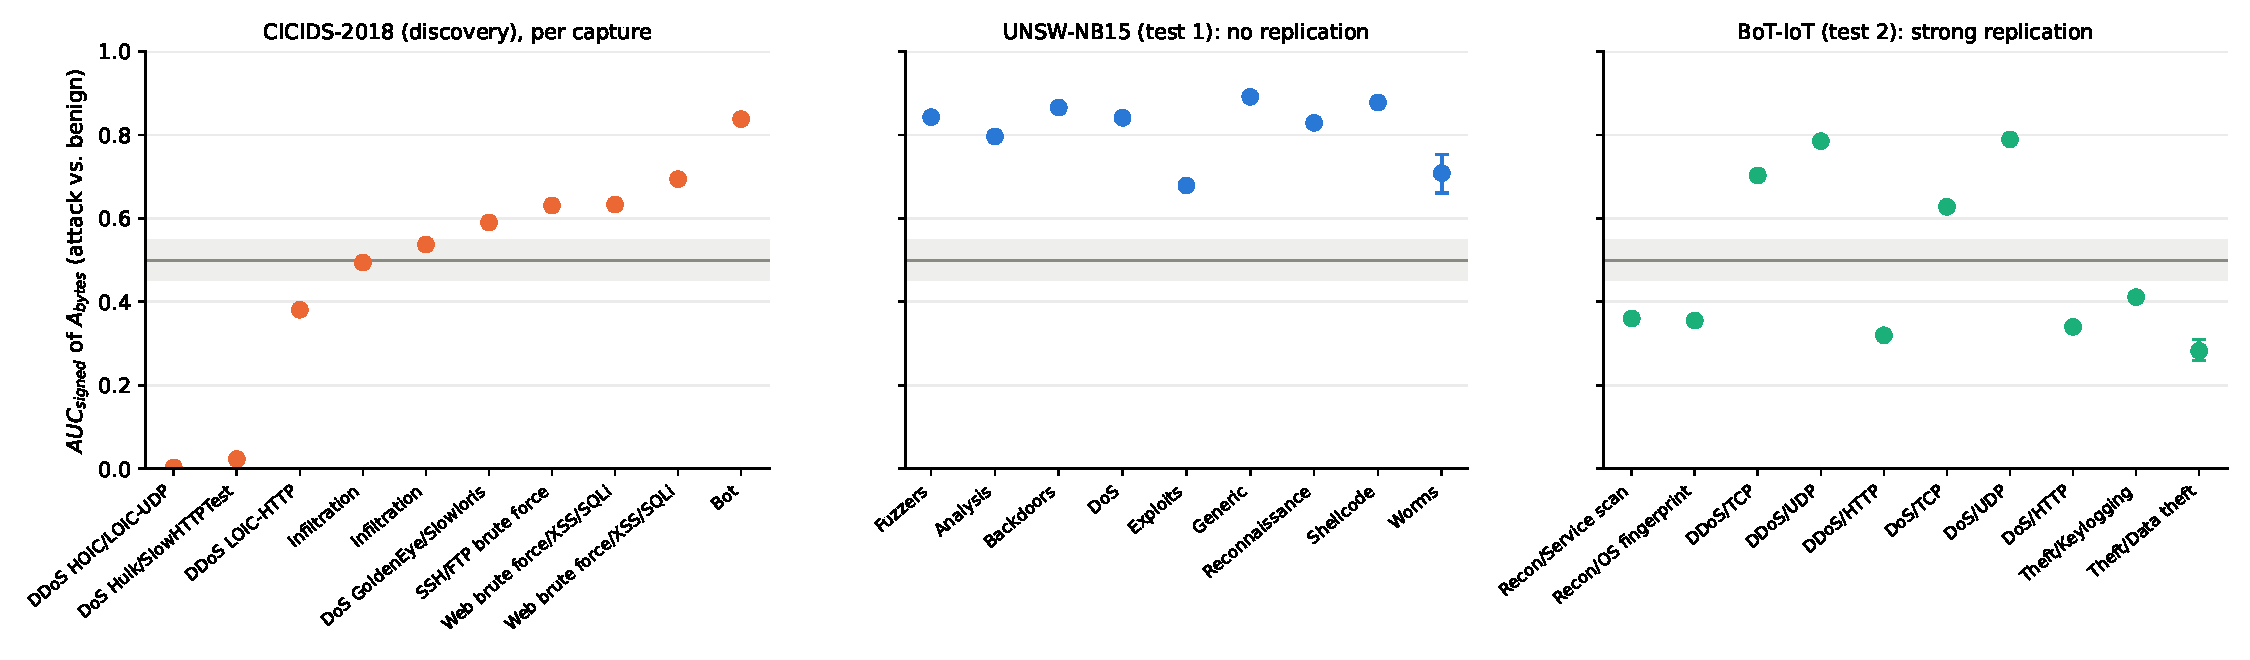
\includegraphics[width=0.7\textwidth]{figures/fig_orientation.pdf}
\caption{$AUC_{signed}$ of $A_{bytes}$: CICIDS-2018 discovery (left; one point per capture against its own benign flows), UNSW-NB15 (center) and BoT-IoT (right) with preregistered flow-level 95\% CIs, which overstate precision under host-pair dependence (Table~\ref{tab:bot}).\label{fig:orientation}}
\end{figure}

\subsection{H3 external tests}\label{sec:h3res}

\textbf{UNSW-NB15: NO REPLICATION.} All nine families were confidently positive on both features (Fig.~\ref{fig:orientation}, center; $A_{bytes}$ 0.679--0.891), the deduplicated population gave the same verdict. H3-dir failed for DoS (0.841). Post hoc, most attack flows receive no reply (0.985 of Generic and 0.777 of DoS flows, against 0.107 of Normal), and 11.5\% of the Normal flows involve an attacker host. Removing them from the reference \emph{raised} every family's $AUC_{signed}$ by 0.072 to 0.097 with all nine still positive (Table~S6), so the result is conservative with respect to the dataset's labeling. All nine families stayed confidently positive under the host-pair bootstrap (25--40 attack pairs per family, 311 benign pairs), and Holm correction changed nothing.

\textbf{BoT-IoT: STRONG REPLICATION under the frozen rule.} All ten groups were confidently oriented on $A_{bytes}$ with opposite signs: hping3 SYN/UDP floods positive (0.628--0.789); scans, GoldenEye floods and both theft groups negative (0.283--0.411); $A_{packets}$ also met the criterion. H3-env held for all six flood groups and H3-dir for two of seven. The verdict stands; Section~\ref{sec:audits} qualifies it.

\subsection{Post-hoc audits}\label{sec:audits}

\textbf{Dependence (A1), BoT-IoT.} The 9{,}543 benign flows come from 347 host pairs, one holding 25.2\%; each evaluable attack group has 32 attack pairs. Flow-level CIs 0.014--0.018 wide became host-pair CIs 0.27--0.41 wide, and resampling only the benign pairs reproduced 89--99\% of that width. Only 3 of 8 evaluable groups (DDoS/TCP, DDoS/UDP, DoS/UDP) kept a confident orientation under every method (Table~\ref{tab:bot}). Removing the dominant benign pair moved three of the four negative evaluable groups into the near-neutral band (0.454--0.481; DDoS/HTTP stayed at 0.427), and equal host-pair weighting made all eight positive (0.785--0.934). A time-block bootstrap cannot express this uncertainty, so its confident intervals are not an alternative reading.

\begin{table}[!t]
\caption{BoT-IoT, $AUC_{signed}$ of $A_{bytes}$ against all Normal flows: preregistered flow-level and host-pair 95\% CIs, equal-host-pair-weight estimate, estimate without the largest benign host pair, and whether every computable method is confident (A1). n/c: not computable. TCP/UDP: hping3 floods; HTTP: GoldenEye floods.\label{tab:bot}}
\centering\scriptsize
\resizebox{\textwidth}{!}{\begin{tabular}{lrcccccc}
\toprule
Group & $n_{attack}$ & $A_{bytes}$ & Flow CI & Host-pair CI & Pair-wtd & w/o top pair & Confident \\
\midrule
Recon/Service scan   & 1{,}463{,}364  & 0.360 & $[0.351, 0.369]$ & $[0.214, 0.597]$ & 0.869 & 0.481 & no \\
Recon/OS fingerprint & 358{,}275      & 0.355 & $[0.346, 0.364]$ & $[0.200, 0.579]$ & 0.864 & 0.473 & no \\
DDoS/TCP    & 19{,}547{,}603 & 0.703 & $[0.696, 0.710]$ & $[0.583, 0.854]$ & 0.924 & 0.721 & yes \\
DDoS/UDP    & 18{,}965{,}106 & 0.785 & $[0.778, 0.792]$ & $[0.634, 0.921]$ & 0.934 & 0.758 & yes \\
DDoS/HTTP   & 19{,}771       & 0.320 & $[0.312, 0.328]$ & $[0.166, 0.562]$ & 0.785 & 0.427 & no \\
DoS/TCP     & 12{,}315{,}997 & 0.628 & $[0.621, 0.635]$ & $[0.487, 0.804]$ & 0.920 & 0.681 & no \\
DoS/UDP     & 20{,}659{,}491 & 0.789 & $[0.782, 0.797]$ & $[0.641, 0.924]$ & 0.933 & 0.759 & yes \\
DoS/HTTP    & 29{,}706       & 0.340 & $[0.332, 0.349]$ & $[0.178, 0.584]$ & 0.795 & 0.454 & no \\
Theft/Keylogging & 1{,}469   & 0.411 & $[0.401, 0.421]$ & n/c & n/c & 0.549 & not evaluable \\
Theft/Data theft & 118       & 0.283 & $[0.259, 0.308]$ & n/c & n/c & 0.372 & not evaluable \\
\bottomrule
\end{tabular}}
\end{table}

\textbf{Reply conditioning (A2).} Restricting attack and benign flows to answered flows gave positive point estimates for all ten BoT-IoT groups (0.585--0.953; Table~S9), although the UDP-flood answered slices (406 and 537 flows) and the theft groups are too sparse for strong inference; among the adequately supported formerly negative groups (HTTP floods, Recon) the negative orientation disappears. On UNSW-NB15, eight of nine families persist on their answered flows; Analysis is the one collapse (0.796 to 0.506 on 630 answered flows, 23.5\% of the family). BoT-IoT's benign reference is small, synthetic, source-dominated (median $A_{bytes}=+4.49$) and only 47.3\% answered, so its negative orientations are negative relative to it, not in absolute terms. A1 and A2 share flows and reference, so their agreement is one observation.

\textbf{CICIDS-2018 labels (A3).} Each capture value is the attack-count-weighted mean of its labels. The value 0.003 equals $(668{,}461\times0.0005+1{,}730\times1.000)/670{,}191$, the aggregate of HOIC (0.0005) and LOIC-UDP (1.000), dominated by HOIC (99.7\% of its flows); it is not the orientation of one mechanism. Three labels change side between per-capture and pooled references (Table~S11) (HOIC 0.0005 to 0.577, Hulk 0.023 to 0.681, SlowHTTPTest). SlowHTTPTest and FTP-BruteForce have $A_{bytes}=0$ on every flow, so their values reflect only the benign reference. Against the pooled reference HOIC and Hulk are positive on all flows and negative on answered-only flows (0.243, 0.329).


\textbf{Representation (A4), CICIDS-2018 only.} Of 11 well-supported labels, 8 have a confident canonical orientation and two reverse under NetFlow-v2, HOIC (0.577 to 0.223) and Hulk (0.681 to 0.349), each against its own benign reference (Table~S12); six are preserved (LOIC-UDP, LOIC-HTTP, SlowHTTPTest, Slowloris, Bot, FTP-BruteForce), SSH-Bruteforce emerges, GoldenEye and Infilteration are near-neutral in both; two of the preserved (SlowHTTPTest, FTP-BruteForce) are constant-valued and not evidence of stable attack-side orientation. Two of 8 is below the frozen Case~D threshold (5 of 8), so the pre-committed reading is \textbf{Case~C}: the orientation of at least one mechanism differs between the two representation-plus-reference pairs. The comparison changes more than the exporter: the benign references differ (13{,}467{,}970 vs.\ 16{,}635{,}567 flows; byte reply rates 0.697 and 0.931), cannot be capture-matched, and segmentation, byte accounting and possibly labeling change with them (C2). A row-level check found 75.5\% of canonical HOIC and 94.1\% of canonical Hulk flows are short unidirectional zero-payload records with $A_{bytes}=0$, essentially absent under NetFlow-v2, which resembles the attempted-attack and construction artifacts documented for CICFlowMeter~\cite{engelen2021troubleshooting,liu2022errorprevalence}; counting header bytes would push those records further positive, so byte accounting does not explain the reversal.

\subsection{Orientation is not separation}\label{sec:sep}

Sixteen sign changes between two values outside the band occur across the audits (six CICIDS-2018, ten BoT-IoT); that their $AUC_{sep}$ stays at or above 0.55 (0.577--0.777 and 0.585--0.869) holds by construction, and the magnitudes are the information, moving in both directions. Under NetFlow-v2 HOIC's separation rose from 0.577 to 0.777 while Hulk's fell from 0.681 to 0.651. Moves into the band lost separation as well (Table~S13).

% =====================================================================
\section{Discussion}\label{sec:discussion}
% =====================================================================

\paragraph{What the results establish} H2 was rejected; H3 failed on UNSW-NB15 and met the frozen criterion on BoT-IoT, which the audits qualify. None of this supports the claim that attack mechanism determines the sign: H3-dir held for 2 of 7 BoT-IoT predictions, and UNSW-NB15 showed no inversion.

\paragraph{Orientation as a relational measurement} $AUC_{signed}$ compares an attack population with a benign reference through a measurement pipeline, so its sign is a property of all three. Each component moved the sign where tested: reference, dependence and weighting mainly on BoT-IoT (and the reference convention on CICIDS-2018), reply composition on BoT-IoT, and representation only for CICIDS-2018 HOIC and Hulk, together with their own reference. UNSW-NB15 is the counterpoint: its orientation survived the host-pair check in all nine families, persisted under reply conditioning in eight of nine, and rose for all when attacker-involved flows left the reference. A relational measurement is not necessarily unstable, but its sign cannot be assumed to be a property of the attack.

\paragraph{Target response is associative and partly definitional} H3-env remains the best-supported pattern here: it predicted the six BoT-IoT flood groups before those data were seen (they come from two tool families, so this is one or two independent predictions) and is consistent with A2. But a flow without reply bytes has $A_{bytes}\ge0$ by construction (the effect scan detectors exploit~\cite{jung2004portscan}), testbed layout can create single-feature artifacts unrelated to the attack~\cite{flood2024smells}, the reference differs across datasets, tooling, exporter and protocol mix vary together, and the prospective support is one test on one testbed: the evidence associates sign with target response and does not show that it causes it. The mechanism reading is not rehabilitated: ``floods invert'' failed on all four hping3 floods. The precision of the preregistered BoT-IoT intervals was a property of the resampling unit (roughly 73 million flows against 347 benign host pairs), and the ten BoT-IoT groups and nine UNSW-NB15 families each come from one testbed: STRONG REPLICATION is one environment meeting a within-environment criterion.

\paragraph{Implications} A fixed-sign rule learned on one benchmark should not be assumed to keep its direction elsewhere until its orientation has been validated under the target pipeline and against the target benign reference (a rule that sending more than receiving is suspicious fits every UNSW-NB15 family but not CICIDS-2018 LOIC-HTTP).

\paragraph{Limitations} All traffic is from testbeds or virtual machines, three environments were examined, and UNSW-NB15 and BoT-IoT are spent as confirmatory sets for H3. The host-pair bootstrap rests on 32 pairs per evaluable BoT-IoT group and 25--40 per UNSW-NB15 family, and percentile intervals from so few clusters can under-cover (Sec.~S3.7). BoT-IoT's benign reference is small, synthetic and concentrated (25.2\% of it from one host pair), and for the scans and GoldenEye floods total size separates the classes as well as or better than direction. The audits are post-hoc, A2 and A4 use point estimates without intervals, exporters count different things, the source-endpoint rule of Argus and NetFlow-v2 is unverified, and nine of ten CICIDS-2018 captures lack IP addresses, so the exporter's direction assignment, which is known to swap source and destination after some TCP timeouts~\cite{engelen2021troubleshooting}, could not be role-checked. Orientation on the corrected CSE-CIC-IDS-2018 data~\cite{liu2022errorprevalence} was not tested, and C2 limits A4 (CICIDS-2018 only).

% =====================================================================
\section{Conclusions}\label{sec:conclusions}
% =====================================================================

The CICIDS-2018 orientation pattern did not replicate on UNSW-NB15 and met the frozen criterion on BoT-IoT (a verdict that depends on the resampling unit and the benign reference). The supported conclusion concerns measurement, not mechanism: signed directional orientation is relational, depending on the benign reference, reply composition, dependence structure and, for CICIDS-2018 HOIC and Hulk, the representation together with its own reference, while separability did not move in lockstep with the sign. UNSW-NB15 shows orientation can also be stable, so the consequence is a validation requirement rather than a prohibition: before a fixed-sign directional feature is carried to a new setting, recompute its orientation against the target pipeline and a named benign reference.

\section*{CRediT authorship contribution statement}
\textbf{David Alexis Garc\'ia Espinosa:} Conceptualization, Methodology, Software, Formal analysis, Data curation, Visualization, Writing -- original draft, Writing -- review \& editing, Supervision, Project administration. \textbf{Misael L\'opez S.:} Conceptualization, Methodology, Validation, Formal analysis, Data curation, Visualization, Writing -- review \& editing. \textbf{Emilio Malagon:} Conceptualization, Methodology, Validation, Formal analysis, Data curation, Visualization, Writing -- review \& editing. \textbf{Jos\'e I. Naranjo-Guerra:} Conceptualization, Methodology, Formal analysis, Data curation, Visualization, Writing -- review \& editing.

\section*{Funding}
This research received no specific grant from any funding agency in the public, commercial, or not-for-profit sectors.

\section*{Declaration of competing interest}
The authors declare no competing interests.

% TODO(authors): archive a release of the repository with a DOI (e.g. Zenodo) and make it public before submission.
\section*{Data availability}
CICIDS-2018, UNSW-NB15 and BoT-IoT are publicly available from their providers~\cite{sharafaldin2018cicids,moustafa2015unsw,koroniotis2019botiot}. The analysis code, the pre-registration freezes, the confirmatory outputs and a provenance file with the original commit hashes and timestamps are available in a cleaned public repository: \url{https://github.com/Ironsss/signed-flow-orientation}.

\section*{Declaration of generative AI and AI-assisted technologies in the manuscript preparation process}
During the preparation of this work the authors used Claude (Anthropic; Claude Code) to support the drafting and editing of the text, to evaluate some ideas, and to assist in writing and reviewing analysis code and project documentation, and Codex (OpenAI) as an independent reviewer of the methods. After using these tools, the authors reviewed and edited the content as needed and take full responsibility for the content of the published article.

\section*{Acknowledgements}
% TODO(authors): add individuals (advisors, colleagues) if desired.
The authors thank the Tecnologico de Monterrey for the academic training that provided the foundations for this work.

\def\bibfont{\scriptsize\linespread{0.92}\selectfont}\setlength{\bibsep}{0pt}
{
\bibliographystyle{elsarticle-num}
\bibliography{references}
}
\end{document}
